\addcontentsline{toc}{chapter}{Контрольная работа 1}
\chapter*{Контрольная работа 1}

\addcontentsline{toc}{section}{Вариант 1}
\section*{Вариант 1}

\subsubsection*{1}

\textit{Задание.} В сундуке лежат 10 красных, 6 синих и 4 зелёных пуговицы.
Найдите вероятность того, что две наугад вынутые пуговицы будут разного цвета.

\textit{Решение.}
Опишем пространство элементарных исходов: $ \Omega = \\ = \left\{ \left( x, y \right), \, x, y \in \right.$ красный, синий, зелёный\}\}.
Нужно выбрать две пуговицы из двадцати, поэтому $ \left| \Omega \right| = C_{20}^2$.

Опишем событие $A =$ \{две наугад вынутые пуговицы будут разного цвета\} $= \left\{ \left( x, y \right) in \Omega: \, x \neq y \right\} $.
Выберем сначала одну красную пуговицу --- $C_{10}^1$, а затем --- одну синюю --- $C_6^1$.
По правилу умножения есть $C_{10}^1 \cdot C_6^1$ способов вынуть одну красную и одну синюю пуговицу.
Второй случай: одна из пуговиц красная, другая --- зелёная --- $C_{10}^1 \cdot C_4^1$.
Третий случай: одна из пуговиц синяя, другая --- зелёная --- $C_6^1 \cdot C_4^1$.
По правилу суммы имеем, что $ \left| A \right| = C_{10}^1 \cdot C_6^1 + C_{10}^1 \cdot C_4^1 + C_6^1 \cdot C_4^1$.

Тогда вероятность равна
$$P \left( A \right) =
\frac{ \left| A \right| }{ \left| \Omega \right| } =
\frac{C_{10}^1 \cdot C_6^1 + C_{10}^1 \cdot C_4^1 + C_6^1 \cdot C_4^1}{C_{20}^2}.$$

\subsubsection*{2}

\textit{Задание.} Подбросили 10 игральных кубиков.
Найдите вероятность того, что единица выпала хотя бы на двух кубиках, если известно, что она выпала хотя бы на одном кубике.

\textit{Решение.}
Опишем пространство элементарных событий:
$ \Omega = \\
= \left\{ \left( x_1, x_2, \dotsc, x_{10} \right): \,
x_i \in \left\{1, 2, 3, 4, 5, 6 \right\}, \,
i =
\overline{1, 6} \right\} $.
На каждом кубике может выпасть число от одного до шести (6 вариантов), поэтому $ \left| \Omega \right| = 6^{10}$.

Рассмотрим событие $A =$ \{единица не выпала ни на одном кубике\}.
На каждом кубике может выпасть число от одного до пяти.
Таких вариантов есть $5^{10}$.
Тогда вероятность события $A$ равна
$$P \left( A \right) =
\frac{ \left| A \right| }{ \left| \Omega \right| } =
\frac{5^{10}}{6^{10}}.$$

Тогда событие $ \overline{A} =$ \{единица выпала хотя бы на одном кубике\} имеем вероятность
$$P \left( \overline{A} \right) =
1 - P \left( A \right) =
1 - \frac{5^{10}}{6^{10}}.$$

Рассмотрим событие $B =$ \{единица выпала хотя бы на двух кубиках\}.
Рассмотрим пересечение событий $ \overline{A} \cap B =$ \{единица выпала хотя бы на двух кубиках\} $= B$.
Рассмотрим противоположное событие: $ \overline{B} =$ \{единица выпала ровно на одном кубике\} $
\cup $ \{единица не выпала ни на одном кубике\} $= B_1 \cup A$.
Найдём количество способов выпадения цифр на кубиках, которые ему удовлетворяют.

$B_1 =$ \{единица выпала ровно на одном кубике\}.
Нужно выбрать 1 кубик из десяти, на котором выпала единица --- это $C_{10}^1$.
На остальных десяти кубиках может быть любое число от двух до шести --- $5^9$.
По правилу умножения $ \left| B_1 \right| = C_{10}^1 \cdot 5^9$.
Вероятность этого события равна
$$P \left( B_1 \right) =
\frac{ \left| B_1 \right) }{ \left| \Omega \right| } =
\frac{C_{10}^1 \cdot 5^9}{6^{10}}.$$

Тогда вероятность события $B$ равна
$$P \left( B \right) =
P \left( A \right) + P \left( B_1 \right) =
\frac{5^{10}}{6^{10}} + \frac{C_{10}^1 \cdot 5^9}{6^{10}} =
\frac{5^{10} + C_{10}^1 \cdot 5^9}{6^{10}}.$$

Условная вероятность события $B$ при условии, что событие $ \overline{A}$ произошло, равна
$$P \left( \left. B \right| \overline{A} \right) =
\frac{P \left( \overline{A} \cap B \right)}{P \left( \overline{A} \right) } =
\frac{P \left( B \right)}{P \left( \overline{A} \right) } =
\frac{ \frac{5^{10} + C_{10}^1 \cdot 5^9}{6^{10}}}{1 - \frac{5^{10}}{6^{10}} }.$$

\subsubsection*{3}

\textit{Задание.} Допустим, что в среднем 5 мужчин из 100 и 25 женщин из 10000 являются дальтониками.
Наугад выбранный человек оказался дальтоником.
Какая вероятность того, что это был мужчина?

\textit{Решение.} Рассмотрим событие $A =$ \{наугад быбранный человек оказался дальтоником\}.
Рассмотрим гипотезы: $H_1 =$ \{выбранный человек --- мужчина\}, $H_2 =$ \{выбранный человек --- женщина\}.
Мужчин и женщин в популяции одинаковое количество, поэтому вероятности гипотез равны
$$P \left( H_1 \right) =
\frac{1}{2} =
P \left( H_2 \right).$$
Условные вероятности:
$$P \left( \left. A \right| H_1 \right) =
\frac{5}{100}, \,
P \left( \left. A \right| H_2 \right) =
\frac{25}{10000}.$$
По формуле Байеса
$$P \left( \left. H_1 \right| A \right) =
\frac{P \left( \left. A \right| H_1 \right) P \left( H_1 \right) }{P \left( \left. A \right| H_1 \right) P \left( H_1 \right) +
P \left( \left. A \right| H_2 \right) P \left( H_2 \right) } =
\frac{ \frac{5}{100} \cdot \frac{1}{2} }{ \frac{5}{100} \cdot \frac{1}{2} +  \frac{25}{10000} \cdot \frac{1}{2} }.$$

\subsubsection*{4}

\textit{Задание.} Петя играет в орлянку.
Он начинает игру, имея одну гривну.
Если выпадет орёл, то Петя получает одну гравну, в другом случае --- теряет одну гривну.
Была сиграна 21 игра, после которой Петя остался без денег и без долга.
Найдите вероятность того, что Петя впервые остался без денег именно в последней игре.

\textit{Решение.} На рисунке \ref{fig:4} изображены возможные пути.

\begin{figure}[h!]
  \centering
  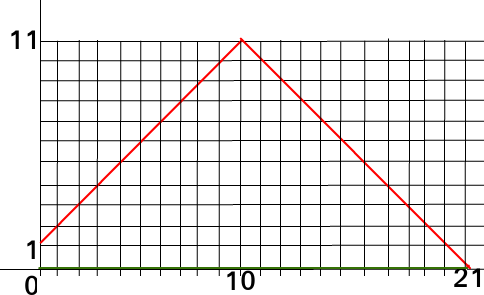
\includegraphics[width=.4\textwidth]{./pictures/t1v1_4.png}
  \caption{Пути}
  \label{fig:4}
\end{figure}

Они ограничиваются красной линией.
Зелёную линию пересекать не можем.
Касаться её можно только в точке $ \left( 21, 0 \right) $.

Перевернём изображение (рис. \ref{fig:41}).

\begin{figure}[h!]
  \centering
  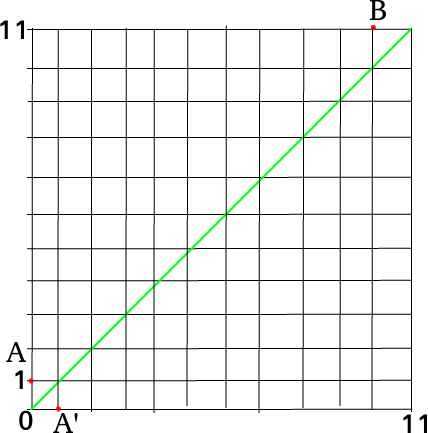
\includegraphics[width=.4\textwidth]{./pictures/t1v1_41.png}
  \caption{Перевёрнутое изображение}
  \label{fig:41}
\end{figure}

Теперь можем ходить направо и вверх.
Всего путей из точки $A$ (начальной) в точку $B$ (конечную) $C_{10+11}^{10} = C_{21}^{10}$.
По методу отражения путей, которые касаются или пересекают диагональ столько, сколько путей из точки $A'$ в точку $B$.
Их $C_{9+11}^9 = C_{20}^9$.
Тогда путей, которые не касаются и не пересекают диагональ $C_{21}^{10} - C_{20}^9$.

А вероятность такого события равна
$$P =
\frac{C_{21}^{10} - C_{20}^9}{C_{21}^{10}}.$$

\subsubsection*{5}

\textit{Задание.} В равнобедренный прямоугольный треугольник с катетами длиной $1$ см наугад бросили точку.
Найдите вероятность того, что расстояние от этой точки до какой-то из вершин треугольника не превышает 0.5 см.

\textit{Решение.} Эта задача на геометрическую вероятность.
Пространство элементарных событий $ \Omega $ --- равнобедренный прямоугольный треугольник с катетами длиной 1.
Его площадь равна
$$S_{ \Omega } =
\frac{1}{2} \cdot 1 \cdot 1 =
\frac{1}{2}.$$
Событие $A =$ \{расстояние от наугад выбранной точки в данном треугольнике до какой-то из его вершин не превышает 0.5\} на рисунке \ref{fig:5} закрашено чёрным цветом.

\begin{figure}[h!]
  \centering
  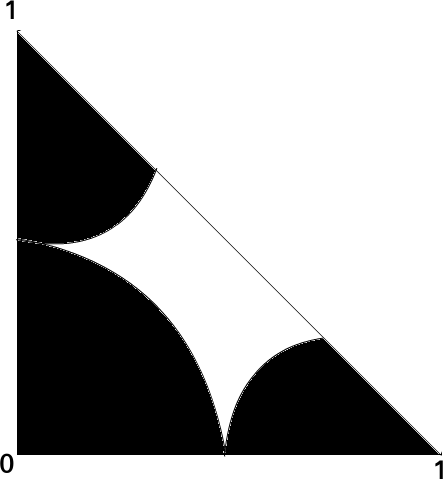
\includegraphics[width=.4\textwidth]{./pictures/t1v1_5.png}
  \caption{Пространство элементарных событий $ \Omega $ и событие $A$}
  \label{fig:5}
\end{figure}

Точки множества $A$ образуют 3 части.
Первая часть --- четверть круга с радиусом 0.5 возле прямого угла.
Его площадь равна
$$S_1 =
\frac{1}{4} \cdot \pi \left( \frac{1}{2} \right)^2 =
\frac{ \pi }{16}.$$

Две остальные части равна.
Их площади можно найти по формуле для площади сектора круга.
Треугольник равнобедренный и прямоугольный, поэтому углы равны $45 \degree$.
Тогда
$$S_2 =
S_3 =
\frac{ \pi \cdot  \left( \frac{1}{2} \right)^2 \cdot \frac{ \pi }{4}}{2 \pi } =
\frac{ \pi }{16 \cdot 2}.$$

Тогда
$$S_A =
S_1 + S_2 + S_3 =
\frac{ \pi }{16} + 2 \cdot \frac{ \pi }{16 \cdot 2} =
\frac{ \pi }{16} + \frac{ \pi }{16} =
\frac{ \pi }{8}.$$

Вероятность этого события равна
$$P \left( A \right) =
\frac{S_A}{S_{ \Omega }} =
\frac{ \frac{ \pi }{8} }{ \frac{1}{2} } =
\frac{ \pi }{4}.$$

\addcontentsline{toc}{section}{Вариант 2}
\section*{Вариант 2}

\subsubsection*{1}

\textit{Задание.} Из множества $ \left\{ 1, 2, 3, 4, 5 \right\} $ независимо друг от друга выбирают число $ \xi $ и число $ \eta $.
Найдите вероятность того, что число $ \xi^2 - \eta^2$ делится на 2.

\textit{Решение.}
Пространством элементарных исходов является
$ \Omega = \\
= \left\{ \left( \xi, \eta \right): \, \xi, \eta \in \left\{ 1, 2, 3, 4, 5 \right\} \right\} $.
На каждом из двух мест может стоять любая из данных пяти цифр, поэтому $ \left| \Omega \right| = 5^2$.

Рассмотрим событие $A = \left\{ \left( \xi, \eta \right) \in \Omega: \, \left( \xi^2 - \eta^2 \right) \vdots 2 \right\} $.
Его наступлению способствуют такие пары чисел:
$ \left( 1, 1 \right), \left( 2, 2 \right),
\left( 3, 3 \right), \left( 4, 4 \right),
\left( 5, 5 \right), \left( 2, 4 \right),
\left( 4, 2 \right), \\
\left( 1, 3 \right), \left( 3, 1 \right), \left( 1, 5 \right), \left( 5, 1 \right), \left( 3, 5 \right), \left( 5, 3 \right) $.
Этих пар 13, поэтому $ \left| A \right| = 13$.

Тогда вероятность события равна
$$P \left( A \right) =
\frac{ \left| A \right| }{ \left| \Omega \right| } =
\frac{13}{5^2} =
\frac{13}{25}.$$
